\lab{Application}{Stochastic Cake-Eating Problem}{Stochastic Cake-Eating Problem}
\newcommand\ve{\varepsilon}

\objective{In this section we study the stochastic cake-eating problem with both normal and AR(1) shocks.}

\section*{Infinite Horizon, Stochastic, i.i.d.}\label{SecRecProbInfinHorStochiid}

In practice, dynamic programming problems often involve some level of uncertainty.  For example as time progresses prices may change, resources may vary, or preferences themselves may change.  In this lab, we reexamine the cake eating problem, this time allowing for uncertainty.

We consider again the problem of opimizing a sequence of decisions over an infinite time horizon.  We assume that the individuals preferences fluctuate each period according to some "shock" $\ve$, meaning $\ve$ is a random variable.  We assume that the $\ve$ are identically and independently distributed (i.i.d).  In effect, this means the probabilities associated with the $\ve$ are the same for any time $t$ and do not depend on each other.  We assume for now that the $\ve$ are distributed normally with mean $\mu$ and variance $\sigma^2$.  The Bellman equation can be easily rewritten in the following way to incorporate the uncertainty,
\begin{equation*}\label{stoch_Bellman}
   V\left(W,\ve\right) = \max_{W'\in[0,W]}\: \ve u\left(W - W'\right) + \beta E_{\ve'}\left[V\left(W',\ve'\right)\right] \quad\text{where}\quad \ve \sim \text{N}(\mu,\sigma^2)
\end{equation*}
where $E$ is the unconditional expectations operator over $\ve$.  Note that now the value function is a function of two variables.  It represents the value of entering the period with $W$, the amount of cake, and a preference shock of $\ve$.  For example, in a period where the realization of $\ve$ is higher, we will get more value from the cake eaten in the current period.  Because we do not know the value of the shock in the next period $\ve'$, we consider only the expected value for future time.

It turns out, we can solve this problem in a manner similar to the infinite horizon deterministic cake-eating problem considered in the Value Function Iteration lab.  It is worth noting that in this case, computationally the value and policy functions will be two dimensional as they will depend on both $W$ and $\ve$.

In order to deal with $\ve$ computationally, we would like to represent it as a vector of possible values it could take along with the corresponding probabilities that it takes each of those values.  However, $N(\mu,\sigma^2)$ is a continuous distribution so we cannot represent every value $\ve$ could take.  We need a discrete distribution that approximates $N(\mu,\sigma^2)$.

To do this we can think of breaking the distribution $N(\mu,\sigma^2)$ up into bins with endpoints $v_1,v_2,\ldots, v_K$.

\begin{figure}[h!]
\label{stoch1_fig1}
\begin{center}
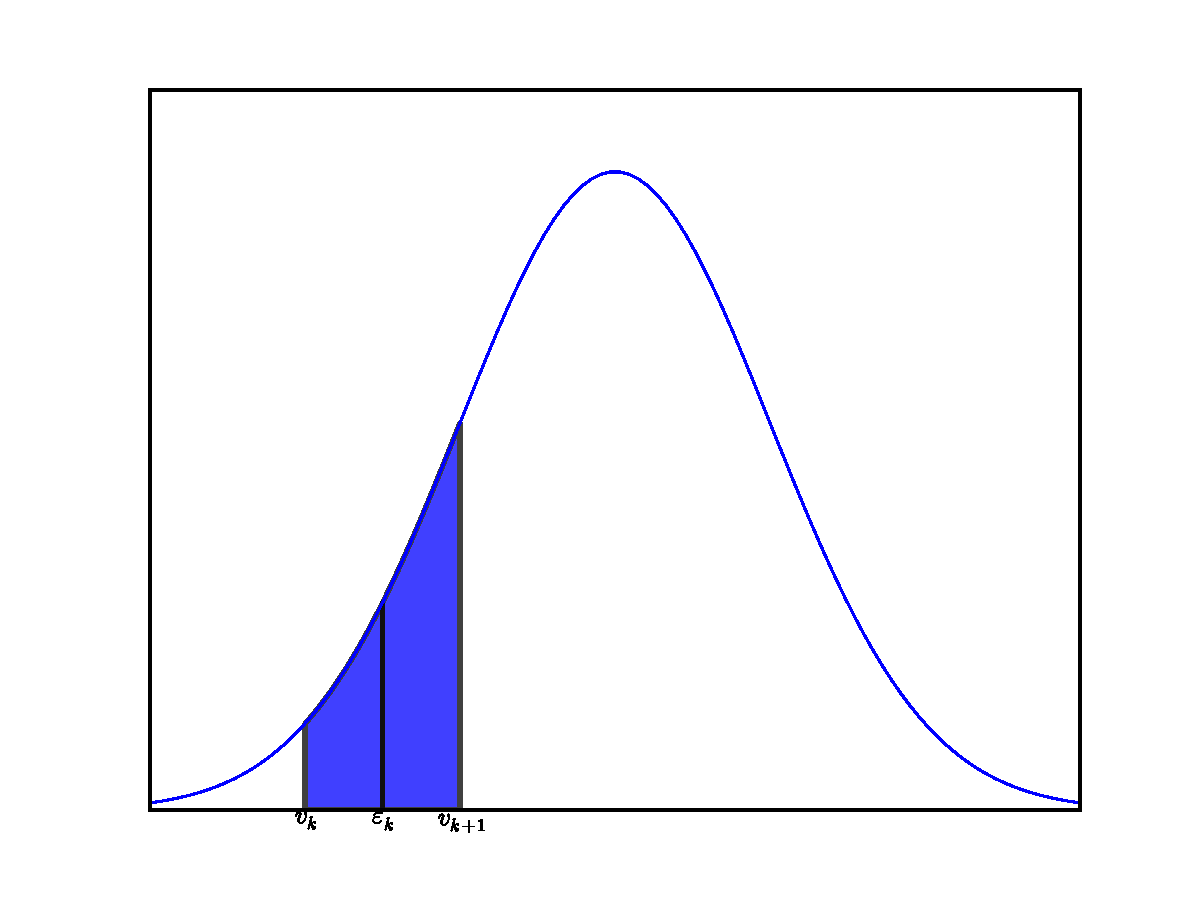
\includegraphics[width = \textwidth]{discnorm.pdf}
\end{center}
\caption{Discretization of $N(\mu,\sigma^2)$.  We approximate $P(\ve = \ve_k)$ by the area of the shaded region.}
\end{figure}

We can then associate $\ve_k$ with the area under the curve from $v_k$ to $v_{k+1}$.  In python we can find the area using the function norm.cdf in the stats package.  The cdf function gives the area under the curve from minus infinity to a specified value.  For example, in the following code, eps is the area under the curve from 0 to 1.

\begin{lstlisting}[style=python]
from scipy import stats as st

mu = 0
sigma = 1
eps = st.norm.cdf(1,mu,sigma) - st.norm.cdf(0,mu,sigma)
\end{lstlisting}

In general, it is sufficient to take our points $\ve_k$ ranging from $\mu - 3\sigma$ to $\mu + 3\sigma$.

\begin{problem}
Write a function called discretenorm that accepts an integer representing the number of discrete points desired, a mean, and a standard deviation and returns a 1 by N vector of values ranging from $\mu - 3\sigma$ to $\mu + 3\sigma$  and a 1 by N vector of the associated probabilities.  Plot the approximation of $N(0,1)$ using 7 points.
\end{problem}

Now that we have a discrete distribution for $\ve$, we can solve for the value and policy functions determined by \eqref{stoch_Bellman}.

\begin{problem}
Complete the following steps to solve the problem described above.
\begin{enumerate}
   \item First we establish our approximation of $\ve$ using the discretenorm function created in Problem 1. Let $\sigma^2 = 0.25$ and $\mu=4\sigma$ (This way the shocks, $\ve$, are always positive.) Use $K=7$ equally spaced points to approximate $N(\mu,\sigma^2)$ so that $\ve$ is a $K$-length row vector.  Using the function discretenorm from problem 1, generate the probability distribution $\Gamma$ for $\ve$. This should be a $K$-length row vector whose entries indicate $P(\ve = \ve_k)$

   \item As in the Value Function Iteration lab, assume that the vector of possible cake sizes is $W$ with $N=100$ equally spaced values between 0 and 1.  Represent the value function as a matrix with each row corresponding to different values of $W'$ and each column corresponding to different values of $\ve'$. Initialize the value function to an $N$ by $K$ matrix of zeros.  Assume that the period utility function is $u(c)=\sqrt{c}$, and that the discount factor is $\beta = 0.9$.


   \item In order to evaluate the value function equation we need to compute $\ve u(W-W')$ for all values of $\ve,W,W'$.  Thus $\ve u(W-W')$ will be represented by a three-dimensional array of size $N\times N\times K$.  This can be achieved using the tile function.  For example, if $u(W-W')$ is represented by the $N\times N$ matrix util\_grid, and eps is the vector of $\ve$ values, then we could create the $\ve u(W-W')$ matrix by the following:

       \begin{lstlisting}[style = python]
       util3 = sp.tile(util_grid[:,:,sp.newaxis],(1,1,K))
       eps_grid = eps[sp.newaxis,sp.newaxis,:]
       eps_util = eps_grid*util3
       \end{lstlisting}

       The input (1,1,K) tells sp.tile to repeat util\_grid K times in the third dimension.  Note we have to put util\_grid[:,:,sp.newaxis] in order to have a three-dimensional input since util\_grid is only two dimensional.

       As in the Value Function Iteration Lab, we replace negative entries in $W-W'$ by 0.

   \item We also need to compute $E_{\ve'}\Bigl[V_k\left(W',\ve'\right)\Bigr]$.  The expected value is simply
       \begin{equation*}
       E_{\ve'}\Bigl[V_k\left(W',\ve'\right)\Bigr] = \sum_k \Gamma(k)V_k(W',\ve_k')
       \end{equation*}  The result is an $N\times 1$ vector that gives the value for each $W'$.  However we need an $N\times N\times K$ array to add to $\ve u(W-W')$.  Since the expected value does not depend on $W,\ve$, we tile the vector to create a 3D array that is constant along the $W$ and $\ve$ dimensions.

   \item We can now compute the value function contraction
     \begin{equation}\label{EqContractStochiid}
      V_{k+1}\left(W,\ve\right) \equiv C\Bigl(V_k\left(W,\ve\right)\Bigr) \equiv \max_{W'\in[0,W]}\: \ve u\left(W-W'\right) + \beta E_{\ve'}\Bigl[V_k\left(W',\ve'\right)\Bigr].
      \end{equation}
        Before doing so, replace the entries of $\ve u\left(W-W'\right) + \beta E_{\ve'}\Bigl[V_k\left(W',\ve'\right)\Bigr]$ that corrsepond to $W-W' < 0$ with a large negative number (e.g. $-10^{10}$) so they will not be chosen in the maximization.

   \item As we iterate on the value function equation, we need a norm
    \begin{equation*}
        \delta_k = \norm{V_k\left(W,\ve\right) - V_{k-1}\left(W,\ve\right)}
    \end{equation*}
    that measures the distance between the two value functions to determine convergence.  Compute the norm using the scipy function scipy.linalg.norm.  Iterate on the contraction until $\delta_k < 10^{-9}$.

   \item Make a 3-D surface plot of the policy function for the converged problem $W' = \psi\left(W,\ve\right)$ which gives the value of the cake tomorrow as a function of the cake today  and the taste shock today.  Do the same for the value function.

\end{enumerate}
\end{problem}

\begin{figure}
    \centering
    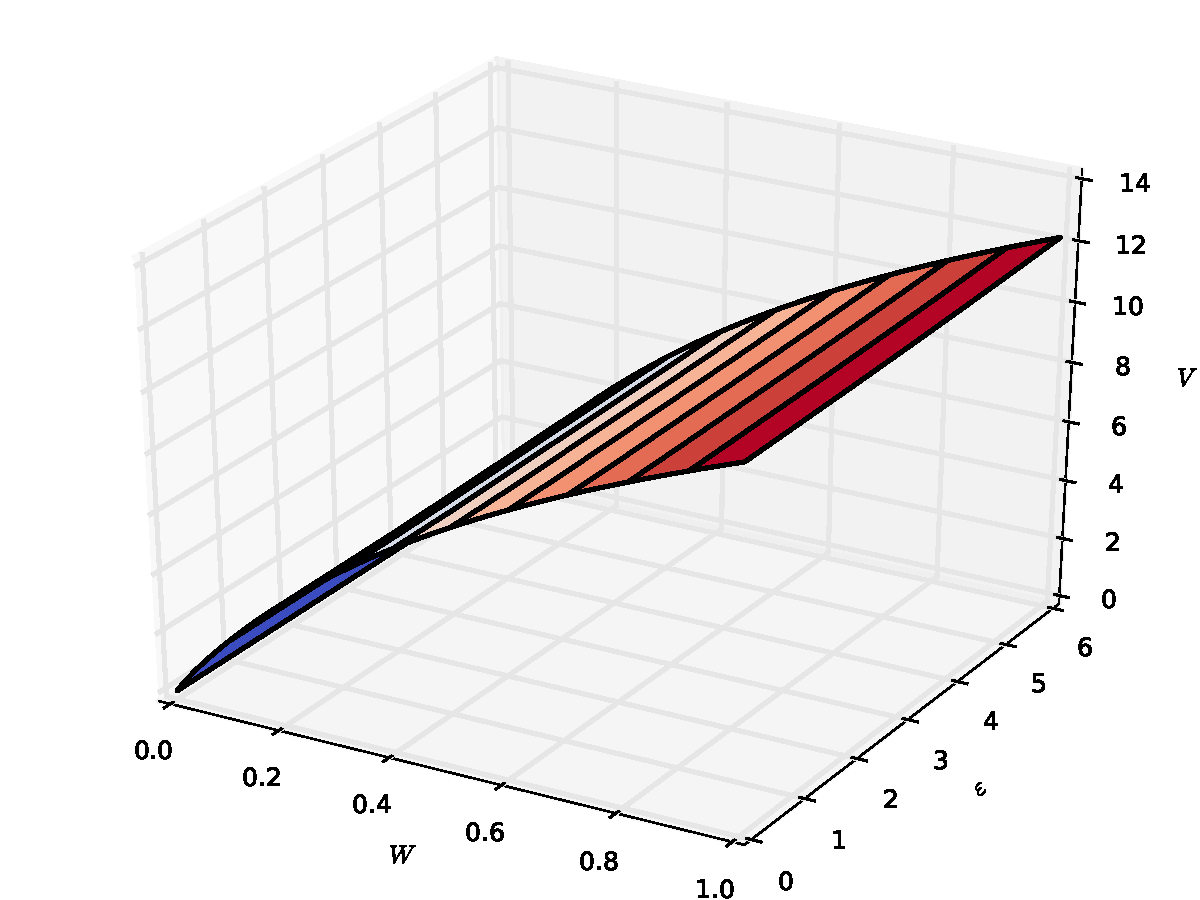
\includegraphics[width = \textwidth]{stoch_value.pdf}
    \caption{3D surface representing the value function for the Stochastic Cake-Eating problem.}
\end{figure}

\section*{Infinite Horizon, Stochastic, AR(1)}\label{SecRecProbInfinHorStochAR1}

In the previous example we assumed that the shocks at time $t$ were independent of what happened in previous periods.  Often a shock may depend on recent events.  We will assume now that the shocks are persistent, meaning preferences in the current period are more likely to be close to what they were in the previous period.  We can characterize the persistence by what is called an autoregressive process of order one, denoted AR(1).  Such a process is defined as follows.
\begin{equation}\label{EqAR1shock}
   \ve' = (1-\rho)\mu + \rho\ve + \nu' \quad\text{where}\quad \rho\in(0,1) \quad\text{and}\quad \nu\sim N(0,\sigma^2)
\end{equation}

Essentially, instead of allowing the shocks to have a mean which is independent of the past, the mean is now a weighted average (weighted by $\rho$) of some $\mu$ and the previous realization of the shock, $\ve$.  As it turns out, we can approximate this process by thinking of it like a Markov Chain. This means we need to determine a discrete set of points representing possible values of $\ve$ and a Markov transition matrix that gives the probabilities of moving from one value of $\ve$ to another.  There are methods for determining the discrete approximation of $\ve$ with a Markov transition matrix.  The methods are beyond the scope of this section, but you can use the file tauchenhussey.py to implement them in the next problem.

The Bellman equation becomes the following, in which the only change from the i.i.d. shock case is that the expectations operator is now conditional on the current shock $\ve$.

\begin{equation*}
   V\left(W,\ve\right) = \max_{W'\in[0,W]}\: \ve u\left(W - W'\right) + \beta E_{\ve'|\ve}\left[V\left(W',\ve'\right)\right]
\end{equation*}
where $\ve'$ is distributed according to \eqref{EqAR1shock}. Let $\Gamma(\ve'|\ve)=\text{Pr}\left(\ve_j'|\ve_i\right)$ where $\ve_j'$ is the value of the shock in the next period and $\ve_i$ is the value of the shock in the current period.  In other words, $\Gamma(\ve' | \ve)$ is the Markov transition matrix.

The solution to this problem is of the same type as that in the i.i.d. case since the only difference is the probability distributions of the $\ve$.

\begin{problem}
\begin{enumerate}
   \item Use the file tauchenhussey.py to approximate the AR(1) process for $\ve$ from \eqref{EqAR1shock} as a Markov chain. The provided Python function tauchenhussey.py will produce a vector of length $M$ for the support of $\ve$ and an $M\times M$ transition matrix $\Gamma(\ve'|\ve)=\text{Pr}\left(\ve_j'|\ve_i\right)$ where each element in row $i$ and column $j$ represents the probability of the shock $\ve_j'$ next period given the current shock is $\ve_i$. As inputs to tauchenhussey.py, let $M=7$, the mean of the process $\mu=4\sigma$, $\rho = 1/2$, $\sigma=\sqrt{\sigma^2}=1/2$, and $basesigma=(0.5+\frac{\rho}{4})\sigma + (0.5 - \frac{\rho}{4})*\frac{\sigma}{\sqrt{1-\rho^2}}$.

  \item Solving this version of the problem should be very similar to the i.i.d. case completed in problem 2.  The most significant difference is that now we need to compute the conditional expectation
      \begin{equation}
      E_{\ve'|\ve}\left[V\left(W',\ve'\right)\right].
      \end{equation}
      In this case, the expectation is two-dimensional since it depends on both $W'$ and on $\ve$.  The expectation can be computed by matrix multiplying $V(W',\ve')\Gamma(\ve' | \ve)'$ where the last "$'$" represents transposing $\Gamma$.  Again we will need an $N\times N\times K$ array, so we tile the result $K$ times representing that the expectation is constant along $W$.

  \item Solve for the optimal policy by Value Function Iteration.  Plot the value function and policy function surfaces.


\end{enumerate}
\end{problem} 